\section{Introductions}

Task Oriented Dialog(TOD) systems interact with users in the form of dialog using natural language, to accomplish user tasks.
The system needs to understand user needs and provide the best possible response to the user.
The task of extracting user intent and goals from conversations by filling belief slots is called Dialog State Tracking (DST)~\cite{wang-etal-2016-inner}.
Using DST and dialog history, the system needs to decide what actions to take and then convey that action in the form of natural language to the user.

Traditional TOD systems were built using a pipeline approach, where each component is created separately and then integrated into the system.
However, with the adaptation of large pretrained language models~\cite{Devlin2019BERTPO,Radford2019LanguageMA},
researchers have moved towards end-to-end systems~\cite{HosseiniAsl2020ASL,Peng2021SoloistBT,Lee2020SUMBTLaRLEN,Yang2020UBARTF,Jeon2021DORATP,Sun2022BORTBA,Yang2022UBARv2TM},
In these systems, the dialog history is fed to the model as input and the output is a cascaded generation~\cite{su2021multi} of the DST, System Actions and System Response.

\begin{figure}[!t]
    \centering
    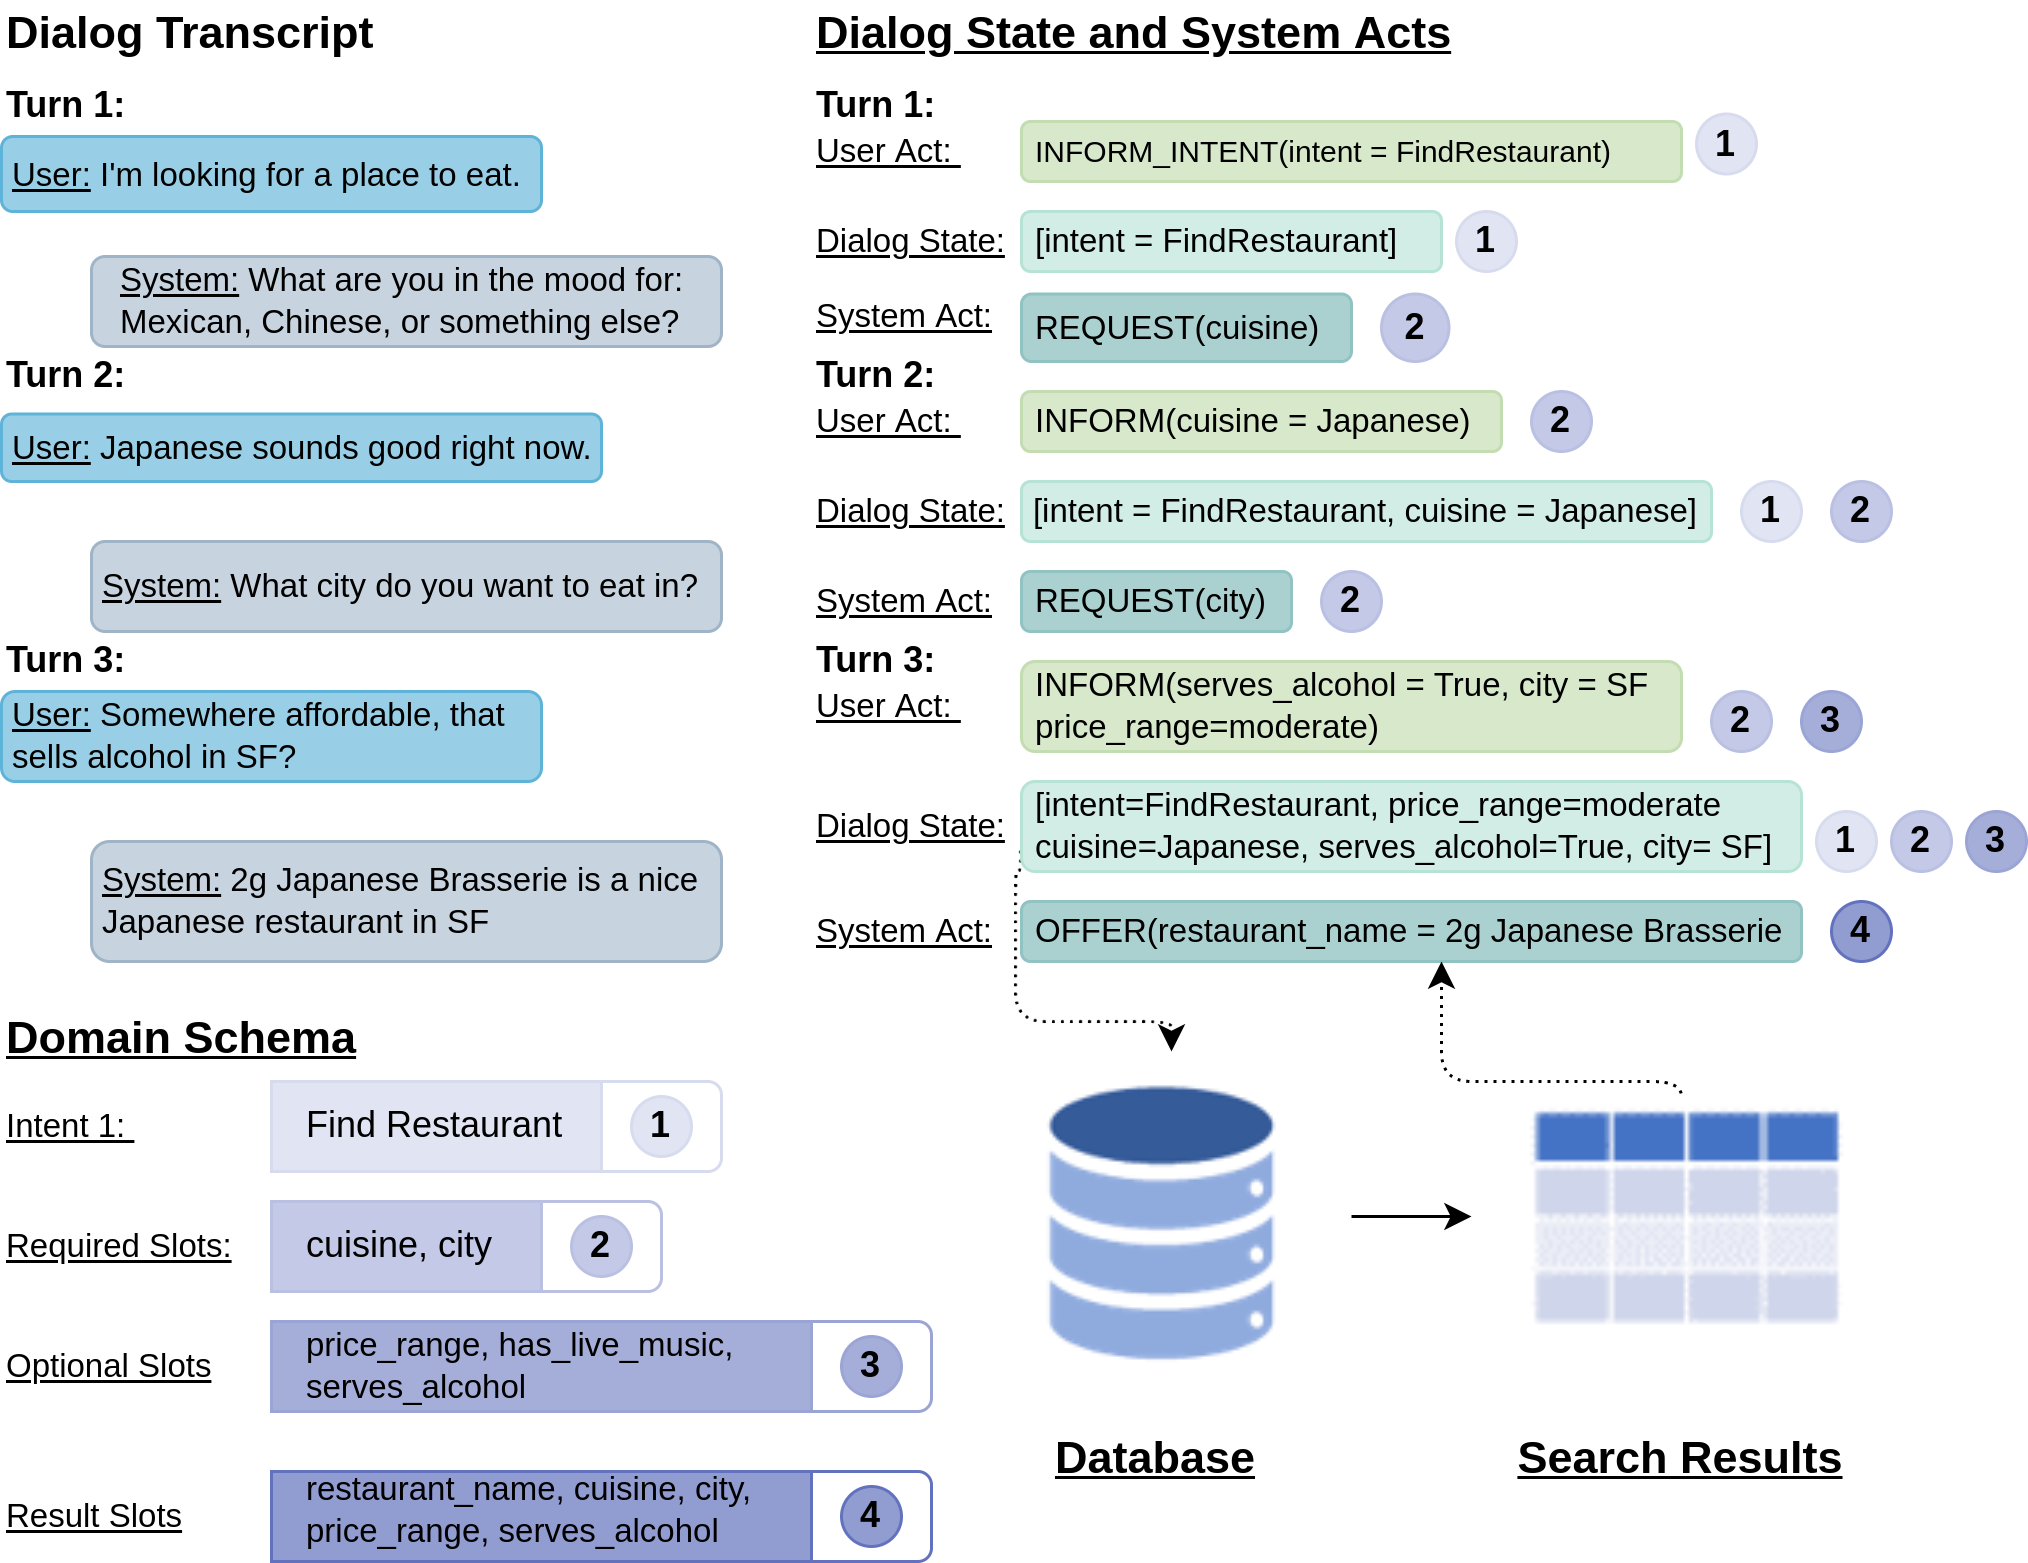
\includegraphics[width=\linewidth]{assets/approach.png}
    \caption{
        Overview of how a Task Oriented System works using schema.
        Given a dialog history consisting of the user and system utterances and the domain schema, for the current turn the dialog state, system actions and system response is generated.
        Parts of the schema that assist in the generation are grouped by similar colors.
    }
    \label{fig:approach}
\end{figure}

\begin{figure*}
    \centering
    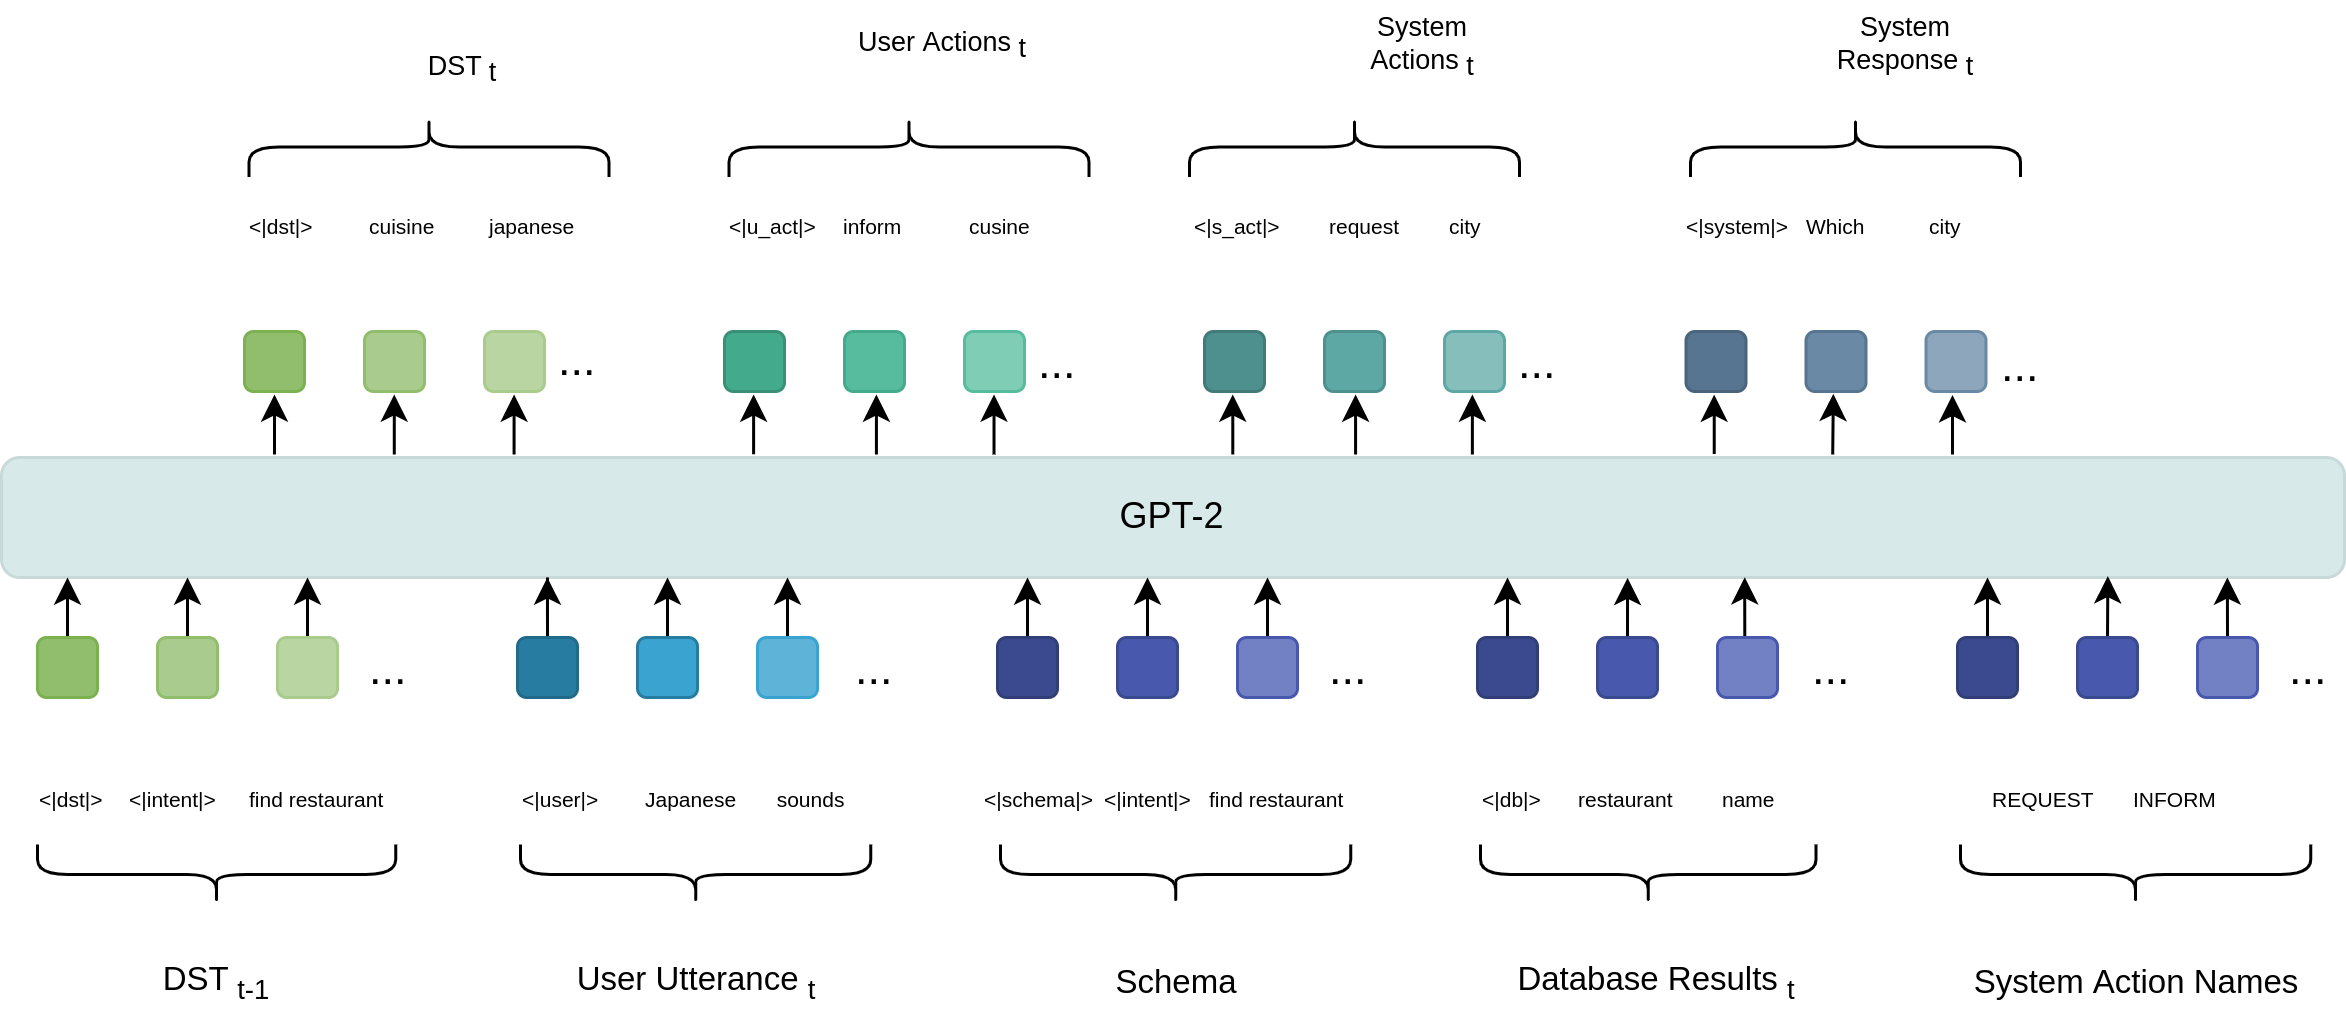
\includegraphics[width=\linewidth]{assets/our_model.png}
    \caption{
        Overview of our approach. A GPT-2 model is fed the dialog state of the previous turn, last user utterance, relevant schemas, database search results and a list of system action names.
        As output, the model autoregressively generates the current dialog state, user actions, system actions and system response.
    }
    \label{fig:our_model}
\end{figure*}



A major drawback of most of these systems is that they fail to generalize to unseen domains. In the real-world setting, ideally a system
should have the capablity to adjust to new domains. Domain knowledge in dialogs can be represented by incorporating schemas, which
lists possible intents, slot names and slot values. An overview of how a TOD system works by incorporating schema is shown in Figure~\ref{fig:approach}.

Some work has been done to create more general systems~\cite{Feng2020ASA,Lee2021DialogueST,Noroozi2020AFA,Mosig2020STARAS,Mehri2021SchemaGuidedPF},
for individual components like the DST, next action prediction and response generation, but there has been no work on generalizable end-to-end systems.

Another drawback in most systems is that they perform poorly in dialogs that have many turns. As the number of turns increases,
the dialog history becomes very long, repetitive and slot values could be updated multiple times in different turns depending on the needs of the user.
This makes it difficult for systems to correctly model long-range semantic dependencies~\cite{sun2022mars}.

To address the aforementioned challenges, we propose a novel Schema Guided Zero-Shot Generalizable End-to-End TOD system using Context Summarization
that outperforms existing state-of-the-art systems. We replace the dialog history with the dialog state as it contains the summary
of the dialog history and is a more compact, efficient and informative representation of the dialog history.
Since the input size is smaller, we can feed additional relevant information to the model, such as the schema, database search results and a list of
system action names, which allows the model to better understand the dialog and generalize to new domains.
We also propose a two step training process, where the first step focuses on understanding the structure of the
data, and the second step focuses on generating the correct output. We conduct experiments on the Schema-Guided Dialog~(SGD) dataset
and provide an ablation study to show the effectiveness of our approach. To the best of our knowledge,
this is the first Zero-Shot End-to-End TOD system designed for the SGD dataset.


